\begin{figure}
  \resizebox{\columnwidth}{!}{%
    \begin{tikzpicture}
      % Actors
      \node[label=Alice + clé $K$] (alice) at (0,0) {
\includegraphics[height=4cm]{img/alice.png}};
      \node[label=Bob + clé $K$] (bob) at (24,0) {
\includegraphics[height=4cm]{img/bob.png}};
      \node[label=Eve sans clé] (eve) at (12,-4) {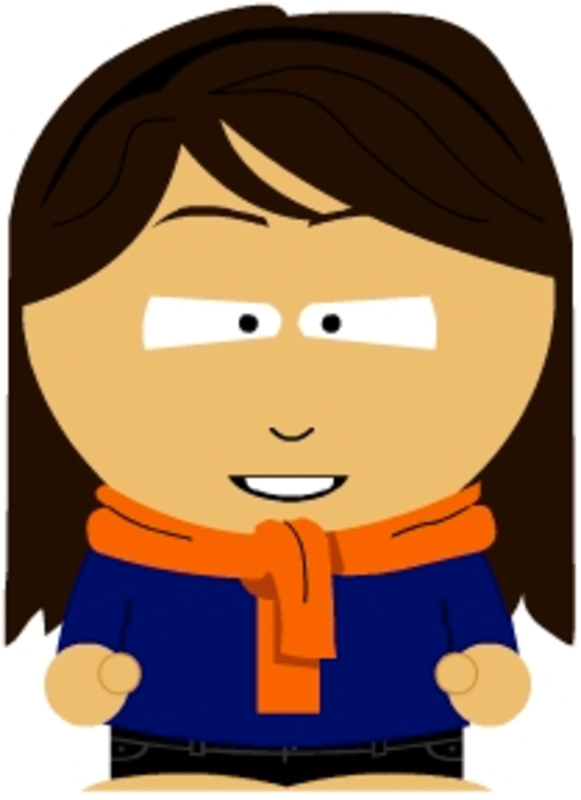
\includegraphics[height=4cm]{img/eve.png}};

      \node[draw] (alice_clear) at (3,0) {Message};
      \node[draw] (cipher) at (12,0) {\#\&*YU*F};
      \node[draw] (bob_clear) at (21,0) {Message};

      \draw[->] (alice_clear.east) -- (cipher) node[near start,above,sloped]{Chiffre avec $K$};
      \draw[->] (cipher.east) -- (bob_clear) node[near end,above,sloped]{Déchiffre avec $K$};

      % Canal
      \draw (8,0) ellipse (0.35 and 0.5);
      \draw (16,-0.5) arc (-90:90:0.5);
      \draw (8,0.5) -- ++(8,0);
      \draw (8,-0.5) -- ++(8,0);
      \node (label) at (12, 1) {Canal de communication non sécurisé};

      \draw[->] (eve.west) -- ++(-1.5,0) -- node[left] {Écoute} ++(0,3.5);
      \draw[->] (eve.east) -- ++(1.5,0) --  node[right] {Modifie} ++(0,3.5);
    \end{tikzpicture}%
  }

  \caption{Chiffrement symétrique avec une clé $K$}
\end{figure}